\newpage
\section{Web-Controlling}
Kennzahlen sind im Controlling angesiedelt. Der Begriff Controlling kommt aus dem englischen. Darunter wird nicht die Kontrolle, sondern die Steuerung des Betriebs verstanden. Das Web-Controlling im speziellen konzentriert sich dabei auf webbasierte Geschäftsmodelle. Zu einem Geschäftsmodell gehört die Formulierung einer Vision die in eine Strategie abgeleitet werden kann, um daraus konkrete Ziele zu definieren. Die Maßnahmen die daraus abgeleitet werden, sollen bei der Zielerreichung helfen. Zur Überwachung dieser Zielerreichung werden Kennzahlen gebildet, die eine Aussage darüber treffen können zu welchem Grad ein Ziel erfüllt ist. Das Web-Controlling liefert dann erst einen Mehrwert, wenn es als Regelkreis verstanden wird bei dem kontinuierlich eine Überwachung der Zielerreichung durchgeführt wird mit deren Hilfe eine erfolgsorientierte Steuerung möglich ist~\footcite[Vgl. ][Seite 83]{Stahl.2009}. 

\subsection{Regelkreis}
Die Voraussetzung für den Einstieg in den Regelkreis sind bereits definierte Key Performance Indikatoren die in eine Web-Scorecard eingetragen werden. Die KPI stellen dabei übergeordnete Kennzahlen dar, die von jedem Unternehmen individuelle definiert werden. Ein klassisches Beispiel wäre die prozentuale Umsatzsteigerung innerhalb eines geplanten Zeitraumes. Die Messung dieser KPI ist möglich, jedoch ist diese Kennzahl nicht in der Lage eine Aussage über Schwachstellen zu treffen. An dieser Stelle wird nun der von William Edwards Deming~\footcite[Vgl. ][Seite 45]{Deming.1986} vorgeschlagene Regelkreis eingesetzt. 

\begin{figure}[H]
	\begin{center}
		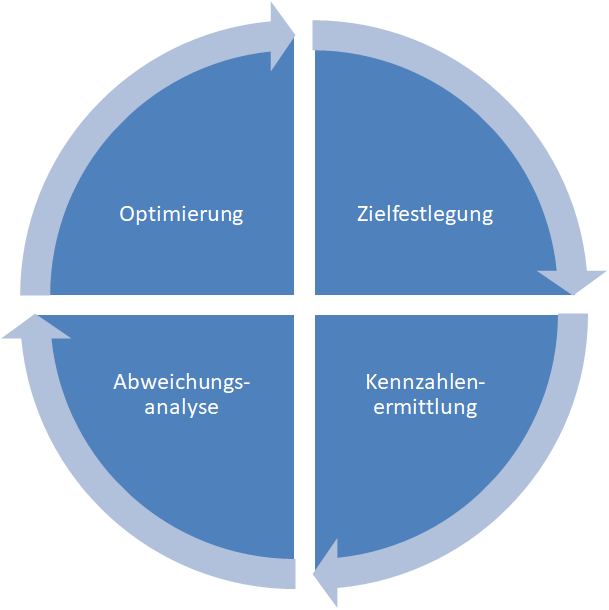
\includegraphics[width=0.9\textwidth]{regelkreis}
		\caption{Web-Controlling Regelkreis in Anlehnung an W.E. Deming}
	\end{center}
\end{figure}

Der erste Schritt besteht darin eine strategische Planung durchzuführen, bei der die Ziele auf die operativen Einheiten heruntergebrochen werden. Im darauf folgenden Schritt beginnt die Umsetzung der Maßnahmen die zur Erreichung der Ziele erarbeitet wurden. Zu diesem Zeitpunkt werden auch die entsprechenden Kennzahlen erhoben. Die eigentliche Messung des Erfolgs findet im darauf folgenden Schritt statt. Bei der Erfolgsmessung ist ein Soll-/Ist-Vergleich notwendig, um eine Aussage darüber treffen zu können zu welchem Grad die Zielerreichung erfüllt worden ist. Sollte eine Kennzahl ein negatives Ergebnis liefern sind Maßnahmen einzuleiten und in kritischen Situation auch Sofortmaßnahmen anzuwenden. Hierfür werden Änderungen am Geschäftsprozess vorgenommen, die im Anschluss erneut durch den Regelkreis überwacht und evaluiert werden müssen.

\subsection{Konversionspfad-Analyse}
Die Analyse der einzelnen Schritte im Bestellprozess wird mithilfe der Konversionspfad-Analyse durchgeführt. Unter Konversion versteht man im Online Marketing die Umwandlung des Status eines Besuchers in einen anderen Status. Konkret sind damit die einzelnen Schritte gemeint, den ein Besucher durchlaufen muss bis zu seinem Kaufabschluss. Innerhalb eines E-Shop bestehen diese einzelnen Schritte aus Webseiten die ein potentieller Kunde dabei durchlaufen muss. Der Weg vom Warenkorb bis zum Bestellabschluss ist der wichtigste Prozess innerhalb eines E-Shop~\footcite[Vgl. ][Seite 152]{Kaushik.2010}, da sich jede Optimierungen innerhalb dieses Prozesses positiv auf den Erfolg auswirkt~\footcite[Vgl. ][Seite 378]{Hassler.2010}. 

\begin{figure}[H]
	\begin{center}
		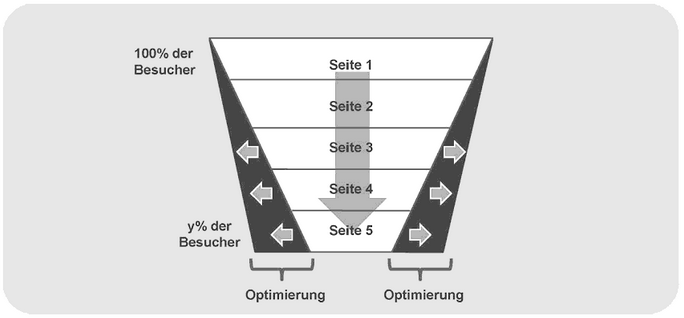
\includegraphics[width=0.9\textwidth]{trichter}
		\caption{Identifikation von Optimierungspotential mit Trichteranalyse~\footcite[Vgl. ][Seite 395]{Hassler.2010}}
	\end{center}
\end{figure}

Die Konversionspfad-Analyse wird auch als Trichteranalyse bzw. Trichterauswertung bezeichnet. Dies ist zurückzuführen auf die Form des Konversionspfades. In der obersten Hierarchie der Analyse befinden sich alle Besucher eines E-Shops. Dort ist es beispielsweise möglich zu analysieren, über welche Seite meine Besucher zu meinem E-Shop gelangt sind. Diese Analyse ist besonders interessant im Zusammenhang mit der Steuerung und Erfolgsmessung von Online-Marketing Kampagnen. Der E-Shop Betreiber hat selbstverständlich auch ein Interesse daran zu messen, welche Produktseiten besonders häufig betrachtet werden. Daher empfiehlt es sich im nächsten Schritt im Konversionspfad die einzelnen Produktseiten zu betrachten. Ein wichtiger Bestandteil im Online-Bestellprozess ist der Start eines Warenkorbs. Dieser signalisiert dem Betreiber, dass ein Kaufinteresse seitens des Kunden existiert. Dieser Teilprozess bildet somit den nächsten Schritt in der Konversionspfad-Analyse ab. Im vorletzten Schritt befindet sich der Kunde im Checkout-Prozess. Dort gibt er seine persönlichen Daten an und schließt somit seine Bestellung ab. Der eigentliche Kaufabschluss wird dann erzielt, wenn der Kunde seine Ware erhalten hat und er mit dem Produkt zufrieden ist. Sollte dies nicht der Fall sein, hat der Kunde beim Online-Einkauf noch die Möglichkeit binnen einer Frist die Ware wieder zurückzusenden. Falls der Kunde sich für eine Rücksendung entscheidet, würde dies zum Ausstieg des Konversionspfad führen und der Kunde würde nicht in der Statistik des letzten Schrittes aufgeführt werden. Nach Hassler~\footcite[Vgl. ][Seite 380-381]{Hassler.2010} können die Ursachen für eine Ausstieg im Konversionspfad durch seine Form analysiert werden. Eine effiziente Konversion führt dazu, dass der Trichter die Form eines Cocktail-Glas annimmt. Ähnelt die Form eher einem Magaritha-Glas, so bekundet der Besucher sein Interesse am Produkt, jedoch fehlen womöglich Details über das Produkt die den Besucher davon abbringen das Produkt in den Warenkorb zu legen. Probleme im Checkout-Prozess bilden beispielsweise die Form eines Weinglas. Demzufolge lässt sich durch die Form eine Aussage über die mögliche Ursache der Konversionshürde ermitteln.

\subsection{Chancen und Risiken}
Nach Abgabe ca. 2 Wochen bis zum Kolloquium.
Die Chancen die sich aus der Implementierung eines Web-Controlling Regelkreis und der aus dem Konversionspfad abgeleiteten Kennzahlen, die im nächsten Kapitel betrachtet werden, sind offensichtlich. Mithilfe des Regelkreises lässt sich stetig der Erfolg eines E-Shops messen und bereits vor auftreten einer Schwachstelle geeignete Gegenmaßnahmen planen. Dies garantiert zwar noch keinen Erfolg, jedoch wird damit eine Steuerung ermöglicht die durch die Qualität der Planung und der Definition von Kennzahlen zu einer höheren Sicherheit beiträgt. Gegenüber E-Shops die nur einen geringen bis gar keinen Aufwand für das Web-Controlling aufbringen, lässt sich somit ein Wettbewerbsvorteil erschließen.
Der Aufwand der betrieben werden muss für ein effektives Web-Controlling sollte dabei nicht unterschätzt werden. Definiert man zu viele oder nicht zielführende Kennzahlen, kann dies zu einer Fehlleitung des E-Shops führen. Die Ursachen für eine Schwachstelle müssen daher gründlich evaluiert werden~\footcite[Vgl. ][Seite 71]{Hassler.2007}. Die Systeme zur Analyse des Benutzerverhaltens zeigen auch nie das exakte Bild der Realität~\footcite[Vgl. ][Seite 35]{Hassler.2010}. Nach Kaushik~\footcite[Vgl. ][Seite 110]{Hassler.2007} müssen daher bei der Datenauswertung mit Abweichungen von bis zu 10% gerechnet werden. Ungeachtet dessen lassen sich durch Vorher-Nachher-Analysen, schlüsse aus dem Trend der Kennzahlen ableiten.

